\chapter{Probleemdefinitie en aanpak}

\section{Probleemdefinitie}
Het doel van dit project is om te onderzoeken hoe het schip Jansje, een historisch transportschip, in de nabije toekomst kan worden verduurzaamd. Hierbij moet rekening gehouden worden met de eisen van de eigenaar van het schip en het Fieldlab Maassluis. Daarnaast moet er gebruikgemaakt worden van groene energie. De opdracht is volbracht als het eindrapport een concreet ontwerpvoorstel bevat voor een duurzame aandrijflijn dat voldoet aan de eisen die gesteld zijn door de eigenaar van Jansje en Fieldlab Maassluis. Concreet betekent dit: 
\begin{itemize}
    \item Een onderbouwde systeemkeuze op basis van een gewogen criteriatabel \cite{Triantaphyllou2000}.
    \item Een energieberekening die aantoont dat de vereiste actieradius haalbaar is.
    \item Een stabiliteitsanalyse die bevestigt dat het schip veilig en efficiënt kan blijven functioneren met het nieuwe systeem.
    \item Een CAPEX/OPEX berekening om te zien of het voorstel financieel haalbaar is
    \item 
    Het voorstel kan voldoen aan de gestelde wet \& regelgeving
\end{itemize}


\section{Belangrijkste uitdagingen \& afbakening}

\subsection{Belangrijkste uitdagingen}
\begin{itemize}

\item \textbf{Wat zijn de financiële parameters voor dit project?} \\
    Bij dit project wordt onder andere gekeken naar duurzame (experimentele) energieopslag. Dit is relatief duur ten opzichte van traditionele energieopslag, dus is het belangrijk om te weten welke financiële eisen er zijn voor dit project. Naast het ophalen van de financiële eisen bij de opdrachtgever, is de methodologische vraag hier: hoe voeren wordt er een betrouwbare CAPEX/OPEX-analyse uit voor een historisch schip met onconventionele systemen?
\item \textbf{Hoe wordt het operationeel profiel van transportschip Jansje het beste bepaald op een representatieve en reproduceerbare manier?} \\
    Om een goede keuze te kunnen maken voor de aandrijflijn en de benodigde energieopslag, is het van belang om rekening te houden met de operationele eisen. Deze eisen bestaan onder andere uit:
    \begin{itemize}
        \item Het benodigde (piek)vermogen.
        \item De benodigde vaaruren per periode.
        \item Hoelang het schip aan wal ligt.
        \item De gemiddelde vaarsnelheid.
        \item nog meer?
    \end{itemize}
    De uitdaging is voornamelijk hoe het vaarprofiel methodisch te bepalen is. Hiervoor wordt gebruik gemaakt van interviews, logboekanalyses en vaarsimulaties gebaseerd op andere schepen. Op deze manier kunnen deze eisen als betrouwbare randvoorwaarden dienen.
\item \textbf{Hoe wordt bepaald welk energieopslagsysteem het meest geschikt is voor Jansje?}\\
    Hierbij wordt gekeken naar een mogelijke nieuwe energieopslag, dit kan bijvoorbeeld een brandstof, generator, batterij of een combinatie zijn. Verschillende duurzame technologieën worden onderzocht en vergeleken met de op dit moment gebruikelijke technologieën. De eisen die bepaald zijn in het programma van eisen worden vertaald naar gewogen criteria om zo op een zo objectief mogelijke en gewogen manier tot een resultaat te komen.
\item \textbf{Hoe wordt bepaald welke aandrijving het best aansluit bij de gekozen energieopslag?}\\
    Transportschip Jansje heeft bij het kiezen van een nieuw energieopslagsysteem ook een nieuwe aandrijving nodig. De keuze voor de aandrijflijn is afhankelijk van het programma van eisen. Daarnaast hebben de technische specificaties en operationele eisen van het energieopslagsysteem een belangrijke keuze in de overweging. De aandrijvingen die voldoen aan deze eisen en specificaties worden vervolgens vergeleken op basis van prestatie aan de hand van een gewogen criteria analyse. 

\item \textbf{Hoe kan het nieuwe systeem theoretisch optimaal geïmplementeerd worden?}\\
    %Hoe kunnen de nieuwe energieopslag en aandrijving het beste geïmplementeerd worden op Jansje? \\
    Hier wordt onderzocht hoe de combinatie van de energieopslag en de aandrijflijn theoretisch optimaal ingebouwd kan worden in transportschip Jansje om de efficiëntie en stabiliteit van het schip te optimaliseren. Het positioneren van de onderdelen in verschillende configuraties creëert fluctuerende technische specificaties zoals bijvoorbeeld de gewichtsverdeling en vaardiepte. Met deze resultaten kan de weerstand en daarmee het vernieuwde benodigd vermogen van het schip worden bepaald. Via iteraties kan vervolgens de optimale configuratie tussen het energieopslagsysteem en de aandrijfmotor worden bepaald om het schip zo efficiënt mogelijk te maken. Om dit te optimaliseren zal een onderzoek worden gedaan aan de hand van Holtrop-Mennen, een CFD (Computational Fluid Dynamics) analyse of een model experiment.
    
\item \textbf{Hoe kan het nieuwe systeem in de praktijk optimaal geïmplementeerd worden?}\\
    Niet altijd is het theoretische optimum haalbaar. Het is dus van belang om een resultaat te hebben dat in de praktijk te realiseren is. Hierbij wordt rekening gehouden met historische aspecten, veiligheid, en technische haalbaarheid.
    
 \item \textbf{Hoe kan de energiecyclus geoptimaliseerd worden?} \\
   Het energetisch opladen en ontladen is van belang om zo min mogelijk (indirecte) uitstoot te krijgen. Daarnaast is het volume van de energieopslag afhankelijk van hoeveel energie er nodig is, waarmee het optimale gebruik van de energie dus resulteert in het laagste volume voor de energieopslag.
   
\item \textbf{Hoe betrouwbaar is het complete systeem?} \\
    Hier wordt onderzocht wat de levensduur is van het nieuwe systeem en naar de onderhoud die daarvoor nodig zal zijn. Dit is zowel financieel, ecologisch als operationeel van belang. \\  
    
\item \textbf{Hoe voldoet Jansje aan de wet- en regelgeving?} \\
    Het kan zo zijn dat bij bepaalde aandrijflijnen het vaartuig niet voldoet aan alle wettelijke eisen. Het is belangrijk dat Jansje aan de wettelijke eisen voldoet of een uitzonderingstatus krijgt, omdat het schip wel gebruikt moet worden.
\end{itemize}
\subsection{Afbakening}
WILLEN WE DIT?

\section{Hoofd- en deelvragen}

\subsection{Hoofdvraag}
\noindent {Welke duurzame aandrijflijn is volgens de commerciële, technische en maatschappelijke eisen het meest geschikt voor het transportschip “Jansje”?} \\


\subsection{Deelvragen}

\noindent De deelvragen zijn direct afgeleid van de hierboven geïdentificeerde uitdagingen en richten zich niet alleen op het ophalen van kennis, maar ook op de methoden waarmee de antwoorden worden verkregen:

\begin{enumerate}
    \item Hoe wordt het operationeel profiel van Jansje op een representatieve en reproduceerbare wijze vastgesteld?
    \item Welk energieopslagsysteem past het best bij Jansje, gegeven de technische parameters, het operationele profiel en  de financiële parameters?
    \item Welk aandrijfsysteem is het meest geschikt voor transportschip Jansje, rekening houdend met het gekozen energieopslagsysteem en het programma van eisen?
    \item Hoe kan de aandrijflijn worden geïntegreerd in de machinekamer van het schip rekening houdend met ruimte, veiligheid, cultureel erfgoed en regelgeving?
\end{enumerate}

\section{Onderzoeksaanpak}
Eerst zal begonnen worden met het vaststellen van het operationeel profiel van Jansje. Hiervoor is de eigenaar geïnterviewd en die gaf alle benodigde informatie. Ook zullen enkele kleine berekeningen gemaakt worden om te bepalen hoeveel vermogen en capaciteit er nodig is voor de hotel-load.
\\\\
Om het energieopslagsysteem voor het schip te kunnen maken, wordt eerst literatuuronderzoek gedaan naar de verschillende mogelijkheden. Met behulp van een excel-model en meerdere criteriatabellen zal de keuze gemaakt worden welk energieopslagsysteem het meest geschikt is. Hiervoor wordt met de Holtrop-Mennen methode de scheepsweerstand berekend, en daarna verder gerekend om het minimaal te installeren motorvermogen te berekenen. Samen met het energieverbruik dat uit het operaitoneel profiel voorkomt, kan nu bepaald worden hoeveel energie constant geleverd moet worden tijdens het varen.
\\\\
Voordat er verder ingegaan wordt op het energieopslagsysteem, wordt eerst nog gekeken naar randvoorwaarden. Deze zijn van belang voor de totale hoeveelheid energie die op het schip opgeslagen moet worden.
\\\\
Vervolgens zal een keuze worden gemaakt voor de meest geschikte energieopslag. Deze keuze wordt gemaakt door middel van modellen, een stroomschema en meerdere criteria.
\\\\
Nu de energieopslag bekend is, kan gekeken worden naar het aandrijfsysteem. Vanuit het operationeel profiel en het gekozen energieopslagsysteem zijn parameters zoals het vermogen en toerental bepaald. Omdat er veel verschillende motoren op de markt zijn, wordt niet gekeken naar één specifieke aandrijving, maar meer naar de parameters waaraan de motor moet voldoen.
\\\\
Als alle onderdelen bekend zijn, wordt door middel van een stabiliteitsberekening gekeken hoe en waar alle onderdelen het best geplaatst kunnen worden om de gewilde eigenschappen te verkrijgen. Tevens wordt gecheckt of het nieuwe gewicht acceptabel is voor het schip.
\\\\
Parallel aan de stabiliteits- en massaberekeningen, is een experiment gedaan met de nog experimentele zeezoutbatterij, om te kijken hoe deze reageert op karakteristieke golfbewegingen waar het in een schip aan blootgesteld wordt.
\\\\
Als laatste wordt afgesloten met meerdere ontwerpen voor de implementatie van het nieuwe systeem in de Jansje. Hiervoor wordt ook rekening gehouden met veiligheid. Hieruit wordt het beste ontwerp gekozen, en deze zal worden voorgelegd aan W. van Baalen als meest geschikte ontwerp om te omplementeren in de Jansje.

\begin{figure}[h]
    \centering
    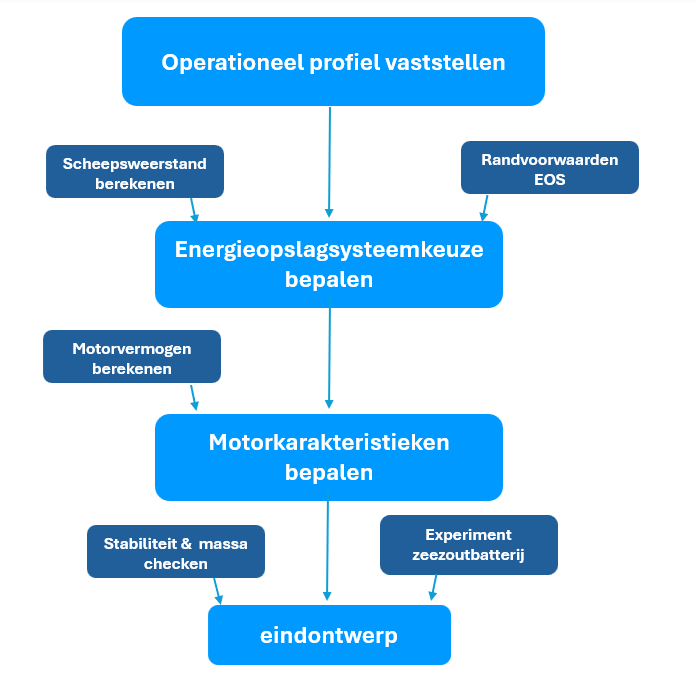
\includegraphics[width=0.8\linewidth]{chart V1.png}
    \caption{Stroomschema van dit project.}
    \label{fig:stroomschema_aanpak}
\end{figure}


\section{Knelpunten, aannames en maatschappelijke aspecten}
\subsection{Knelpunten}
Voor dit project zijn een aantal knelpunten geïdentificeerd.\\

\noindent Allereerst is er beperkt technische data beschikbaar over Jansje. Om deze reden zal er naast de technische data ook data vergaard worden op basis van interviews met de eigenaar en de kapitein, archiefonderzoek en directe opmetingen. Als dit onvoldoende data oplevert, zal worden uitgegaan van referentiewaarden voor vergelijkbare historische binnenvaartschepen uit de literatuur. Dit laatste zal duidelijk aangegeven worden in het verslag.\\

\noindent Ook wordt rekening gehouden met het feit dat stakeholders niet altijd direct zullen reageren. Om te voorkomen dat dit vertraging oplevert, zullen er vroegtijdig plannen gemaakt worden. Daarnaast zal schriftelijke communicatie zo snel als mogelijk verstuurd worden. Bij uitblijven van een respons worden aannames gedaan, gedocumenteerd en voorgelegd tijdens het eerstvolgende contactmoment met de betreffende stakeholders. Eventueel volgt daarna nog een aanpassing in de aannames.\\

\noindent Daarnaast is de verwachting dat er ook gegeken gaat worden naar experimentele technologie, die nog niet is gevalideerd voor nautische applicaties. Aanames die hierbij gemaakt worden, zullen conservatief zijn, en meerdere scenario's zullen worden uitgewerkt.\\

\noindent Als laatste wordt de tijdsdruk bij parallelle deelstudies geïdentificeerd. Om te voorkomen dat deelstudies vastlopen omdat er data en/of conclusies van een parallellopende deelstudies nodig zijn, zullen er wekelijkse meetings plaatsvinden, en duidelijke taken en taakoverdrachten worden gedaan. Als een deelstudie vertraging oploopt, wordt de scope beperkt  tot de voor de energiebalans minimaal benodigde uitvoer. Bijvoorbeeld alleen de kruissnelheid bij de weerstandsberekening in plaats van het volledige vaarprofiel gebruiken.


\subsection{Aannames}
Aannames schrijven die gedaan zijn. BV IN STABILITEIT ETC.


\subsection{Maatschappelijke aspecten}
De gekozen aanpak brengt een aantal maatschappelijke aspecten met zich mee die hieronder worden toegelicht.

\begin{itemize}
    \item \textbf{Veiligheid:} In het ontwerp worden brandveiligheidsmaatregelen meegenomen conform SOLAS-normen \cite{imo_solas_1974} voor kleine schepen. Bij het gebruik van bepaalde brandstofsoorten bestaat explosiegevaar bij lekkage, terwijl batterijsystemen kunnen resulteren in oververhitting en brandgevaar.
    \item \textbf{Duurzaamheid en levenscyclus:} De gebruikte onderdelen in de aandrijflijn worden vergeleken op duurzaamheid. Tevens wordt gekeken naar de levenscyclus van de onderdelen.
    \item \textbf{Ethiek:} Een aantal van de beoogde materialen is schaars en wordt grotendeels gewonnen in landen buiten Europa, waar de werkwijze vaak minder strikt is dan de Europese standaarden \cite{ec_green_claims_2023}  vereisen.
    \item \textbf{Erfgoedwaarde:} Jansje is een historisch schip van grote cultuurhistorische waarde. Ingrijpende veranderingen aan de romp of het interieur kunnen deze waarde aantasten. In overleg met de eigenaar worden aanpassingen zo beperkt mogelijk gehouden; de aandrijflijn en energieopslag worden zo ontworpen dat het historisch karakter van het schip behouden blijft.
\end{itemize}


\section{Leeswijzer}
De rest van het verslag volgt de stappen uit de onderzoeksaanpak. In hoofdstuk 3...